\documentclass[aspectratio=43]{beamer}
% \documentclass[aspectratio=169]{beamer} % proyector 16:9 | Ref:  https://en.wikibooks.org/wiki/LaTeX/Presentations
\usetheme{Boadilla}
\beamertemplatenavigationsymbolsempty %% Sin barra navegación
\usecolortheme{beaver}


%% Spanska!
\usepackage[utf8]{inputenc}
\usepackage{lmodern} % no producia letras en matemático | Ref: https://tex.stackexchange.com/questions/250413/error-when-using-greek-symbol-in-subscript-in-beamer-presentation 
\usepackage[spanish]{babel}
\def\spanishoptions{argentina}

%% inclusión de gráficas
\usepackage{graphicx}	% instalar ghostscript-x para que el dvi muestre los eps
\graphicspath{ {./graphs/} {../figuras/} }
\usepackage{rotating}	% epígrafe rotado


\begin{document}

\title{Curso de ingeniería centrado en código}
\subtitle{Capitalizando lo desarrollado durante el confinamiento}
\author[vbettachini@unlam.edu.ar]{Bettachini, Víctor A.; Real, Mariano A.; Palazzo, Edgardo\\Kowalski, F.; Jara, D.}
%\institute[]{
%	Ingeniería Mecánica, DIIT, UNLaM
%}
\date[2023-09-22]{
	V Encuentro \emph{Mejora de las Estrategias Pedagógicas}%\\22 de septiembre de 2023
}

\usebackgroundtemplate{
  
\includegraphics[width=\paperwidth, height=\paperheight]{diit_titre_background}
}	% unset background % https://tex.stackexchange.com/questions/201013/how-to-include-a-background-image-to-only-one-page-of-a-beamer-presentation

\begin{frame} 
  \titlepage
\end{frame}

\usebackgroundtemplate{
  
\includegraphics[width=\paperwidth, height=\paperheight]{diit_background}
} %% https://mprnotes.wordpress.com/2009/08/14/changing-background-image-of-latex-beamer/


\begin{frame}
	\frametitle{Valorizar el tiempo de docentes y alumnos}
	Licklider (1957): 85\% de ``pensar'' es lo mundano (calcular, dibujar, etc.)
	\pause
	\begin{block}{}
	  \begin{columns}[b]
			\begin{column}{0.3\textwidth}
				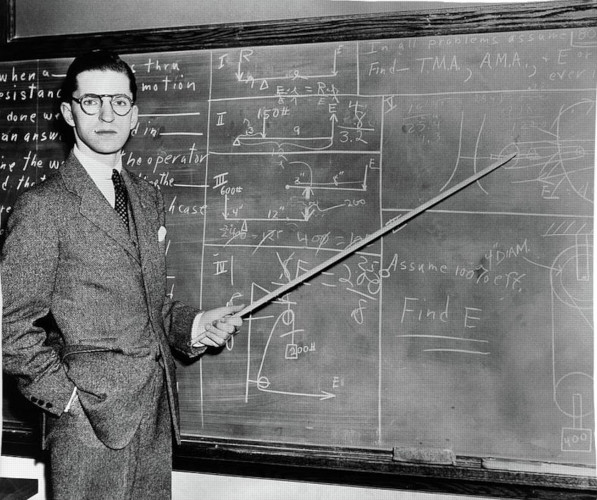
\includegraphics[width= \columnwidth]{1930s-1940s-man-teacher-professor-vintage-images}
			\end{column}
			\begin{column}{0.65\textwidth}
				Aula y práctica: transcripción y reiteración
				\begin{itemize}[<+->]
					\item Memoria \(\xrightarrow{profesor}\) pizarrón/presentación
					\item Pizarrón/presentación \(\xrightarrow{alumno}\) cuaderno
					\item Práctica: \textbf{reiterar} diagramas, cálculos, etc.
					\item Aburrimiento \(\implies \downarrow\) concentración
				\end{itemize}
			\end{column}
		\end{columns}
	\end{block}
	\pause
	\begin{block}{}
	  \begin{columns}[b]
			\begin{column}{0.3\textwidth}
				\includegraphics[width= \columnwidth]{"Screenshot 2023-09-18 at 12-24-03 Google Colaboratory"}
			\end{column}
			\begin{column}{0.65\textwidth}
				\begin{itemize}[<+->]
					\item Ingenio \(\xrightarrow{profesor}\) código en repositorio
					\item Repositorio del curso \(\xrightarrow{alumno}\) propio
					\item Poner en práctica: \textbf{re-utilizar} código
					\item Modificarle resuelve diversas problemáticas
				\end{itemize}
			\end{column}
		\end{columns}
	\end{block}
\end{frame}


\begin{frame}
	\frametitle{Estudiantes de ingeniería deben aprovecharse del código}
	\pause
	\begin{block}{}
		\begin{itemize}[<+->]
			\item Usan calculadora pues \textbf{aprendieron} aritmética en la primaria.
			\item Usarán álgebra computacional pues \textbf{aprobaron} álgebra y análisis.
			\begin{itemize}[<+->]
				\item Enfocarse en nuevas habilidades, no en cálculos automatizables.
				%\item Álgebra y análisis simbólico
				\item Con cálculo numérico resolverán lo imposible en pizarrón/papel.
			\end{itemize}
			\end{itemize}
		% \uncover<4->{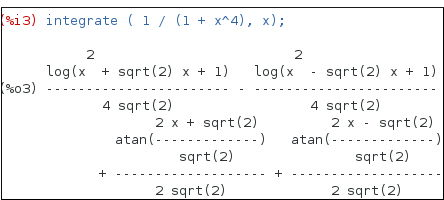
\includegraphics[height= 2cm]{ucarecdn}}
	\only<2>{\includegraphics[height= 2cm]{reglacalculadora}}
	\uncover<3->{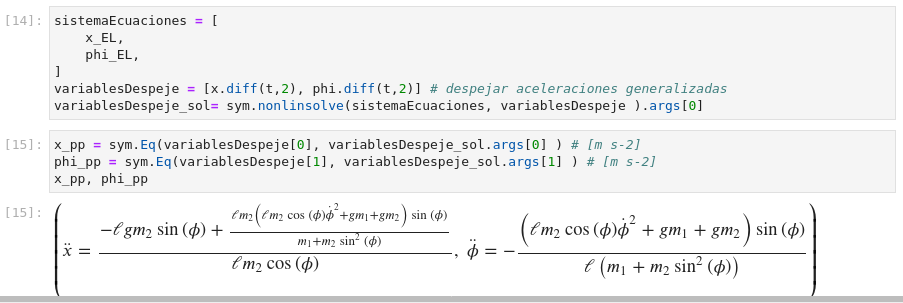
\includegraphics[width= 0.49\textwidth]{hard}}
	\uncover<5->{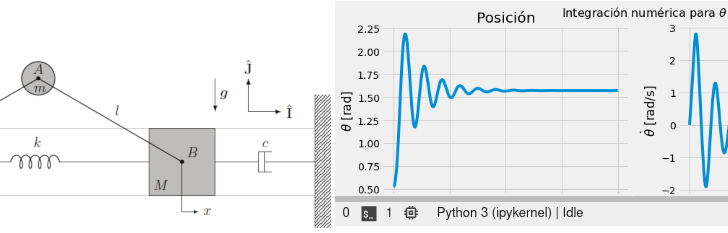
\includegraphics[width= 0.49\textwidth]{impracticable}}
	\end{block}
	\pause
	\begin{block}{}
		Papert (1980) ``El aprendizaje sucede cuando el alumno toma las riendas''
		\begin{itemize}[<+->]
			\item Cierto problema es resuelto por un código provisto por el docente.
			\item El alumno realiza modificaciones para resolver nuevas problemáticas.
			\item Paulatinamente se torna autónomo reutilizando el propio código.
		\end{itemize}
	\end{block}
\end{frame}


\begin{frame}
	\frametitle{Todo el material es editable en línea}
	\pause
	\begin{block}{Cuaderno programable en línea: texto + ecuaciones + código}
		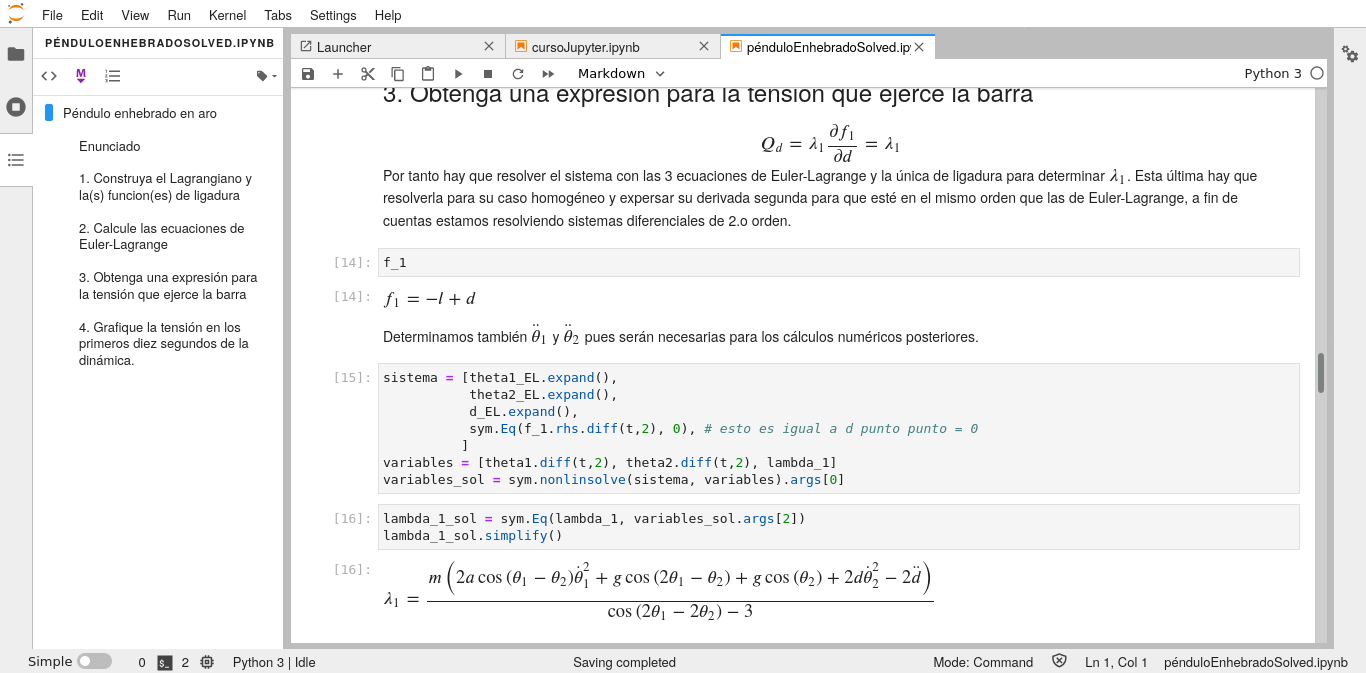
\includegraphics[width= \columnwidth]{screenshot_JupyterLab}
	\end{block}
\end{frame}


\begin{frame}
	\frametitle{Trabajo sincrónico y asincrónico sobre el código}
	\begin{block}{Teoría y ejercicios resueltos en linea en cuadernos programables}
		\begin{itemize}[<+->]
			\item Consultas \textbf{asincrónicas} en línea (24/7) \textbf{públicas} hacia otros alumnos.
			\item Trabajo \textbf{colaborativo remota} en cuadernos multi-usuario.
			\item Al finalizar ejercicios, asistencia docente \textbf{sincrónica individual}
			\item Entrega \textbf{obligatoria} para su corrección \textbf{semanal}.
		\end{itemize}
	\end{block}
	\begin{columns}[b]<1->
    \begin{column}{0.35\textwidth}
			\begin{block}{Aula invertida}
				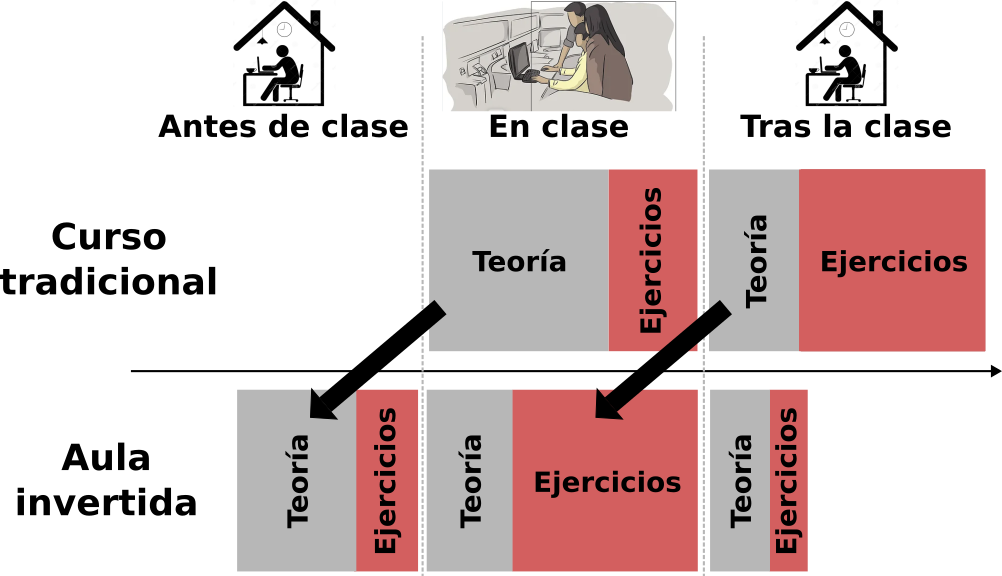
\includegraphics[width= \columnwidth]{diagramaTiempo2.png}
			\end{block}
    \end{column}
    \begin{column}{0.6\textwidth}
			\begin{block}{}
				\begin{tabular}{lll}
					\hline
					Sincrónico & Teoría & Ejercicios\\
					\hline
					Antes & Leer y aplicar & Iniciarles\\
					Durante & Aclarar dudas & Terminarles\\
					% Durante & Aclarar dudas & \begin{tabular}{@{}c@{}}Terminarles\\(semanal)\end{tabular}\\
					Luego & \begin{tabular}{@{}l@{}}Consultas\\adicionales\end{tabular} & \begin{tabular}{@{}l@{}}Correcciones\\del docente\end{tabular}\\
					\hline
				\end{tabular}
			\end{block}
    \end{column}
  \end{columns}
\end{frame}



\begin{frame}
	\frametitle{Asistencia docente y corrección asincrónica}
	\begin{block}{Google Colaboratory: comentando y editando el ejercicio del alumno}
		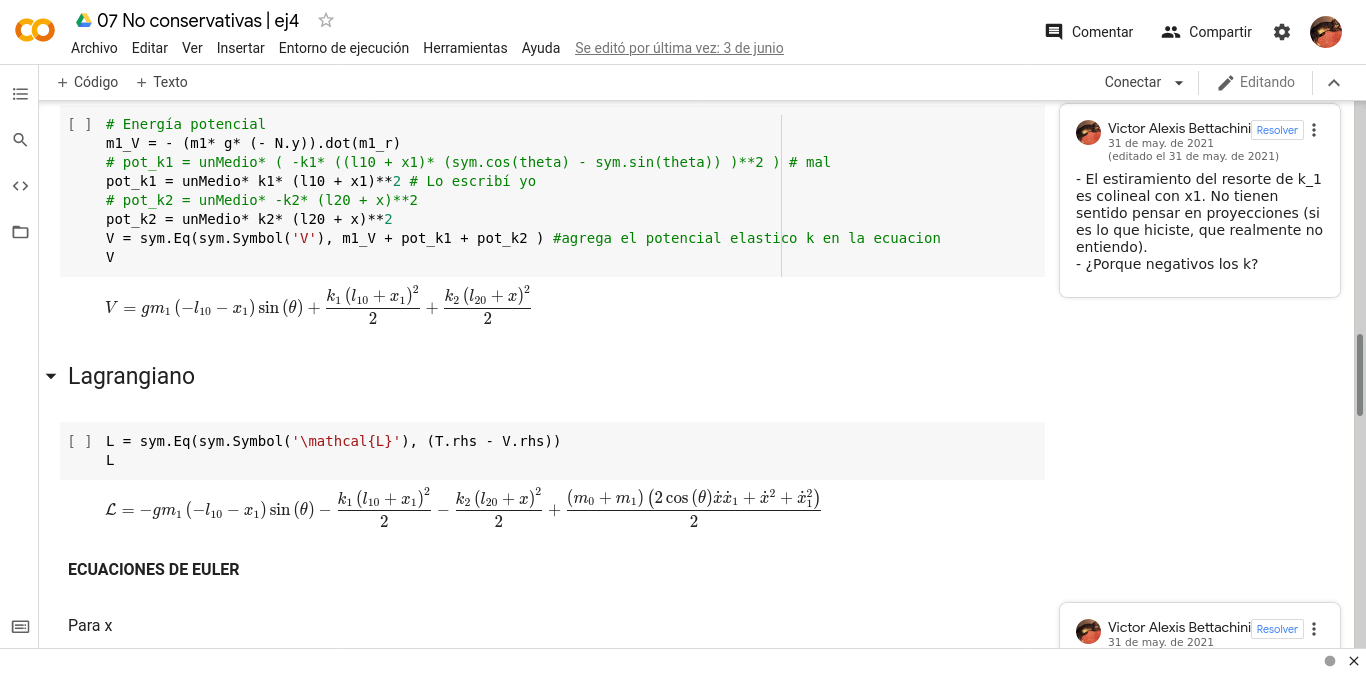
\includegraphics[width= \columnwidth]{comentariosColab}
	\end{block}
\end{frame}


\begin{frame}
	\frametitle{Seguimiento individualizado}
	\begin{block}{Registro del cumplimiento con entregas semanales}
		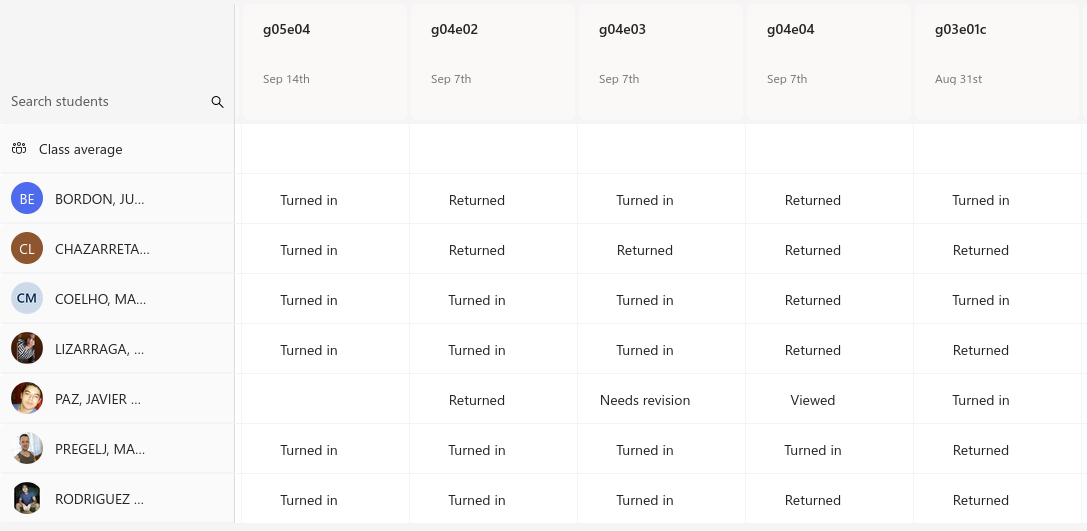
\includegraphics[width= \columnwidth]{seguimiento}
	\end{block}
\end{frame}


\begin{frame}
	\frametitle{Resumiendo}
	\begin{block}{Curso centrado en código}
		\begin{itemize}[<+->]
			\item Teoría: texto + ecuaciones + código ejecutable en cuadernos digitales.
			\item Reforzados con videos propios y bibliografía.
			\item Práctica: reutilización del código del docente.
			\item Ejecución en línea:
			\begin{itemize}[<+->]
				\item Colaboración y corrección remota.
				\item No requiere computadoras en el campus, ni que sean poderosas.
				\item Registro fechado del trabajo del alumno.
			\end{itemize}
		\end{itemize}
	\end{block}
	\begin{block}{Modalidad de aula invertida}
		\begin{itemize}[<+->]
			\item Teoría: énfasis en la lectura autónoma por parte del alumno.
			\item Consultas: asincrónicas y públicas.
			\item Finalizar ejercicios: asistencia personalizada del docente
			%\item Práctica: Docente asiste personalmente cuando más se lo requiere, para finalizar ejercicios.
		\end{itemize}
	\end{block}
\end{frame}
	


\begin{frame}
	\frametitle{Actualidad del proyecto}
	\pause
	\begin{block}{}
		\begin{description}[<+->]
			\item [2023] Retro-alimentación de los alumnos mejoró:
				\begin{itemize}
					\item Apuntes y código en el repositorio.
					\item Metodología ejercitación y evaluación.\\
							Mayor exigencia de ejercicios \(\rightarrow\) mejor respuesta.
				\end{itemize}
			\item [2024] 
				\begin{itemize}
					\item Física II empleará simulaciones provistas por nosotros.
					\item \emph{Prompt engineering}: alumnos generarán código con IA.
				\end{itemize}
			% \item [202x] Difundir la metodología en el DIIT.
		\end{description}
	\end{block}
	\uncover<6->{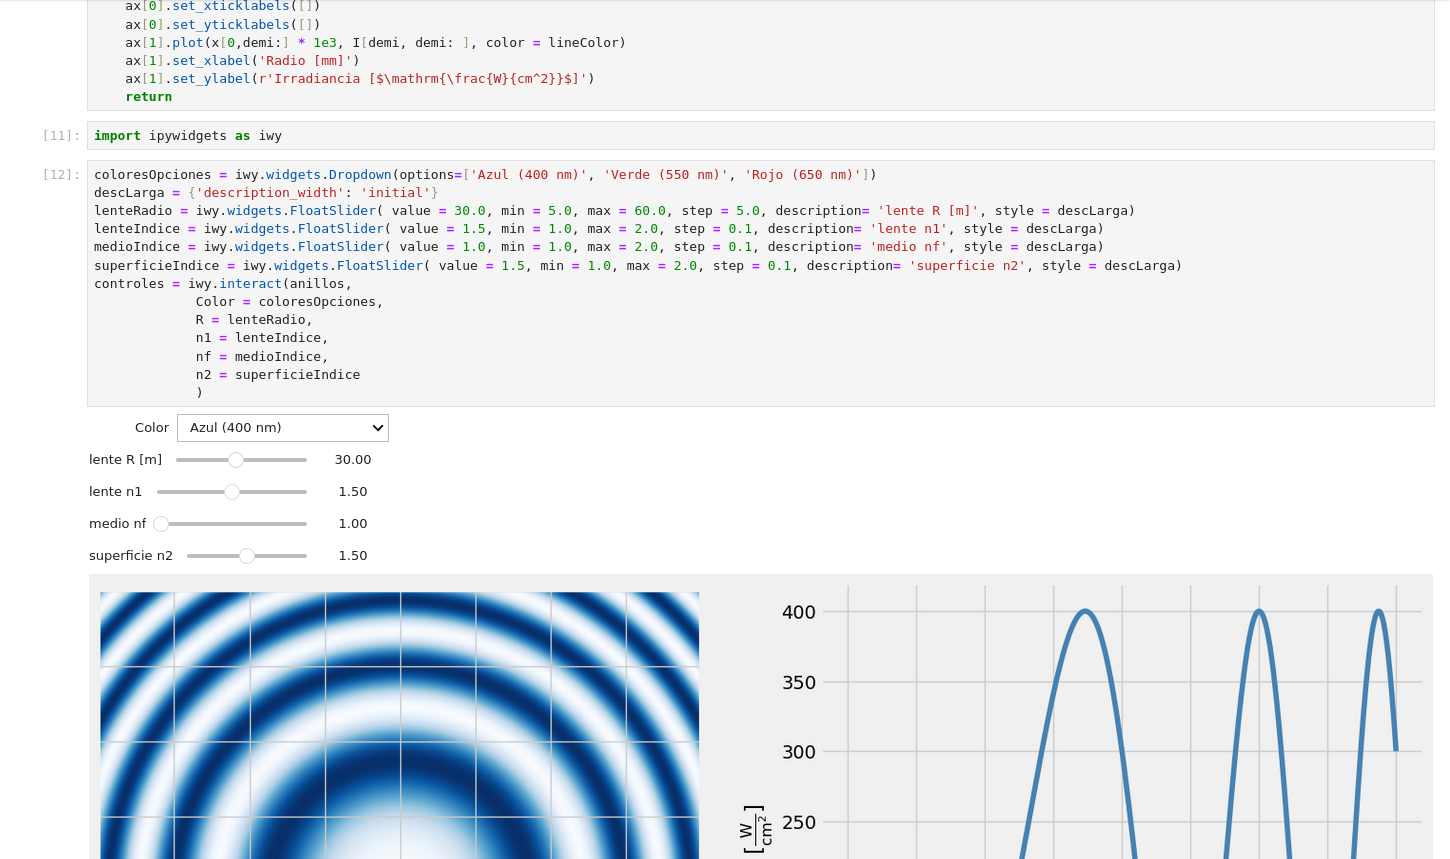
\includegraphics[height= 3cm]{cuñaAnillosN}}
	\uncover<7->{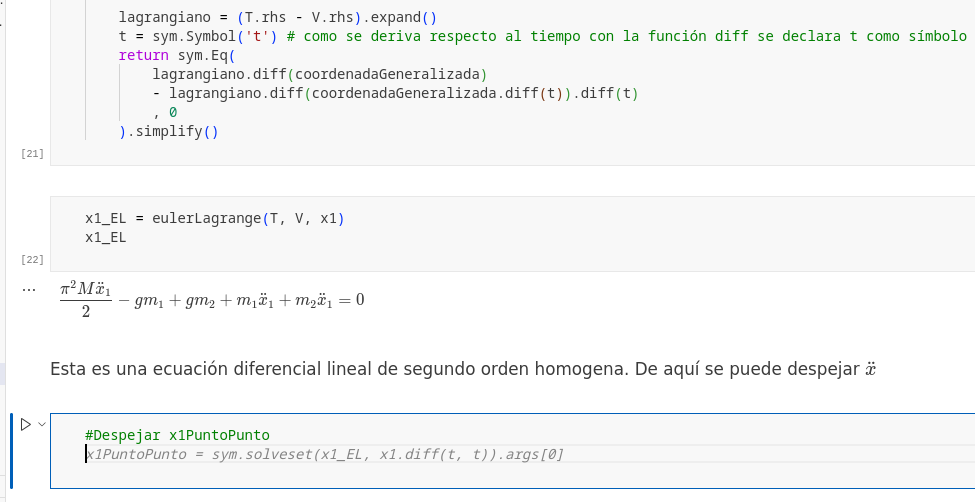
\includegraphics[height= 3cm]{copilot}}
\end{frame}


\end{document}
